\documentclass{article}
\usepackage{../../typesetting/styles/report-zh}
\usepackage{threeparttable} % Add this package for tablenotes environment

\setCJKmainfont{Kaiti SC} % Main Chinese font (Songti)
\setCJKsansfont{Lantinghei TC} % Sans-serif Chinese font
% \setCJKmonofont{Maple Mono NF CN} % Monospaced Chinese font (uncomment if needed)

% Set document information
\title{周报~向嘉豪 (\today)}
\author{向嘉豪}
\date{\today}

\begin{document}

\maketitle

\begin{abstract}
  本周主要工作集中在论文图表的\blue{尺寸调整}与\blue{排版优化},以及论文内容的\blue{学术表达提升}和\blue{重复率检测},最终相似度指数仅为\red{10\%},符合投稿要求。期刊调研后,确定以\red{TCAS-II}为首选投稿目标。
\end{abstract}

\begin{weekplan}
1) \blue{对论文写作进行最后的修改}
2) \blue{准备期刊投稿所需材料}
\end{weekplan}

\section{论文写作}

\subsection{论文修改和查重}

本周对论文的图表进行了\blue{尺寸调整}与\blue{排版优化},确保所有图片和表格在版面中显示合理、清晰。针对论文内容,进一步\blue{提升了学术表达的准确性和逻辑性},对部分段落进行了精炼和重写。随后,使用查重系统对论文进行了重复率检测,\red{最终相似度指数仅为10\%},符合投稿要求。查重结果如图\ref{fig:repetition}所示。

\begin{figure}[ht]
\centering
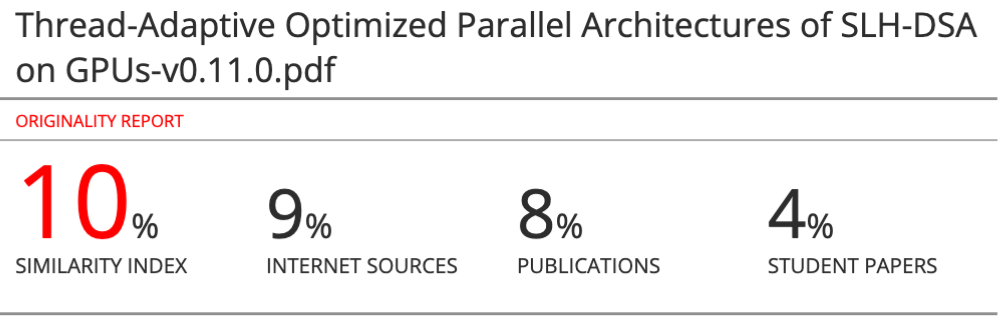
\includegraphics[width=0.5\textwidth]{./fig/reptition.png}
\caption{论文查重结果}
\label{fig:repetition}
\end{figure}

\subsection{期刊选择}

本周针对论文投稿目标期刊进行了系统调研。首先,通过IEEE Xplore等数据库检索了相关\red{IEEE Transactions}系列期刊,并进入各期刊的\blue{在线投稿系统}(如ScholarOne Manuscripts),详细查阅了其\blue{投稿指南}与\blue{作者须知},重点关注了稿件格式、审稿周期、版面费及录用率等核心信息。调研发现,\red{大部分顶级Transactions期刊对Letter/Brief类论文不接受},因此对于本次以\blue{简报(Letter/Brief)格式}为主的稿件,需优先考虑更适合此类论文的次一级期刊。表\ref{tab:journal}对比了当前更具可行性的目标期刊。其中\red{TCAS-II}发表过GPU加速实现AES的文章\cite{Lee2022Jeong}。综上,\red{本次投稿将优先选择TCAS-II作为目标期刊}。

\begin{table}[ht]
\centering
\caption{目标期刊对比分析}
\label{tab:journal}
\resizebox{\textwidth}{!}{
\begin{tabular}{lcccc}
  \toprule
  期刊名称 & 分区 & IF值 & 审稿周期(月) & 年文章数 \\
  \midrule
  \red{\textbf{IEEE Trans. Circuits Syst. II Express Briefs (TCAS‑II)}} & \red{2区} & \red{4.4} & \red{3} & \red{1050} \\
  IEEE Communications Letters  & 3区 & 4.1 & 3 & 680 \\
  IEEE Signal Processing Letters  & 3区 & 3.2 & 3 & 366 \\
  \bottomrule
\end{tabular}
}
{\scriptsize
\caption*{年文章数:为该期刊2024发表的文章数。 审稿周期:查看最新一期的文章,计算从投稿到发表的时间,三篇取平均值。}
}
\end{table}

% Replace standard bibliography commands with conditional version
\printbibliographyifcited[alpha]{../../paper}

\end{document}
